\chapter{ИССЛЕДОВАТЕЛЬСКИЙ РАЗДЕЛ}

\section{Методика проведения экспериментов}

\justifying

Для оценки эффективности разработанной системы семантического поиска проведено экспериментальное сравнение с классическими методами информационного поиска: TF-IDF и BM25. Методика экспериментов включает следующие этапы:

\textbf{1. Подготовка тестового корпуса}

Использован корпус из 116 документов различных форматов (PDF, DOCX, DOC) объемом 42 МБ, включающий научные статьи, технические спецификации и корпоративные документы на русском и английском языках.

\textbf{2. Формирование тестовых запросов}

Подготовлено 10 тестовых запросов различной сложности:
\begin{itemize}
	\item Простые запросы с точным соответствием терминов
	\item Семантические запросы с использованием синонимов
	\item Концептуальные запросы, требующие понимания контекста
	\item Междисциплинарные запросы
\end{itemize}

\textbf{3. Метрики оценки качества}

Для оценки качества поиска использованы следующие метрики:

\textit{Mean Average Precision (MAP)} – средняя точность по всем запросам:
\begin{equation}
	MAP = \frac{1}{|Q|} \sum_{q \in Q} AP(q) \quad,
\end{equation}

\noindent где $AP(q)$ – средняя точность для запроса $q$:
\begin{equation}
	AP(q) = \frac{1}{|R_q|} \sum_{k=1}^{n} P(k) \cdot rel(k) \quad.
\end{equation}

\textit{Mean Reciprocal Rank (MRR)} – средний обратный ранг первого релевантного документа:
\begin{equation}
	MRR = \frac{1}{|Q|} \sum_{q \in Q} \frac{1}{rank_q} \quad.
\end{equation}

\textit{Precision@k} и \textit{Recall@k} – точность и полнота в топ-k результатах.

\textbf{4. Процедура эксперимента}

Для каждого метода выполнены следующие шаги:
\begin{itemize}
	\item Индексация корпуса документов
	\item Выполнение тестовых запросов
	\item Измерение времени выполнения
	\item Расчет метрик качества
\end{itemize}

\section{Сравнение с методом TF-IDF}

Метод TF-IDF реализован с использованием библиотеки scikit-learn со следующими параметрами:
\begin{itemize}
	\item Максимальное количество признаков: 10000
	\item N-граммы: униграммы и биграммы
	\item Минимальная частота документа: 2
	\item Максимальная частота документа: 0.95
\end{itemize}

\textbf{Результаты эксперимента:}

\begin{table}[H]
	\caption{Сравнение Doc2Vec и TF-IDF}
	\begin{center}
		\begin{tabular}{|l|c|c|}
			\hline
			\textbf{Метрика} & \textbf{Doc2Vec} & \textbf{TF-IDF} \\
			\hline
			MAP & 0.823 & 0.547 \\
			\hline
			MRR & 0.891 & 0.621 \\
			\hline
			Precision@10 & 0.756 & 0.512 \\
			\hline
			Recall@10 & 0.834 & 0.543 \\
			\hline
			Среднее время запроса (с) & 0.0234 & 0.0076 \\
			\hline
			Время индексации (с) & 186.3 & 4.7 \\
			\hline
		\end{tabular}
	\end{center}
\end{table}

На рисунке~\ref{fig:quality_metrics} представлено визуальное сравнение метрик качества поиска для различных методов.

\begin{figure}[H]
	\centering
	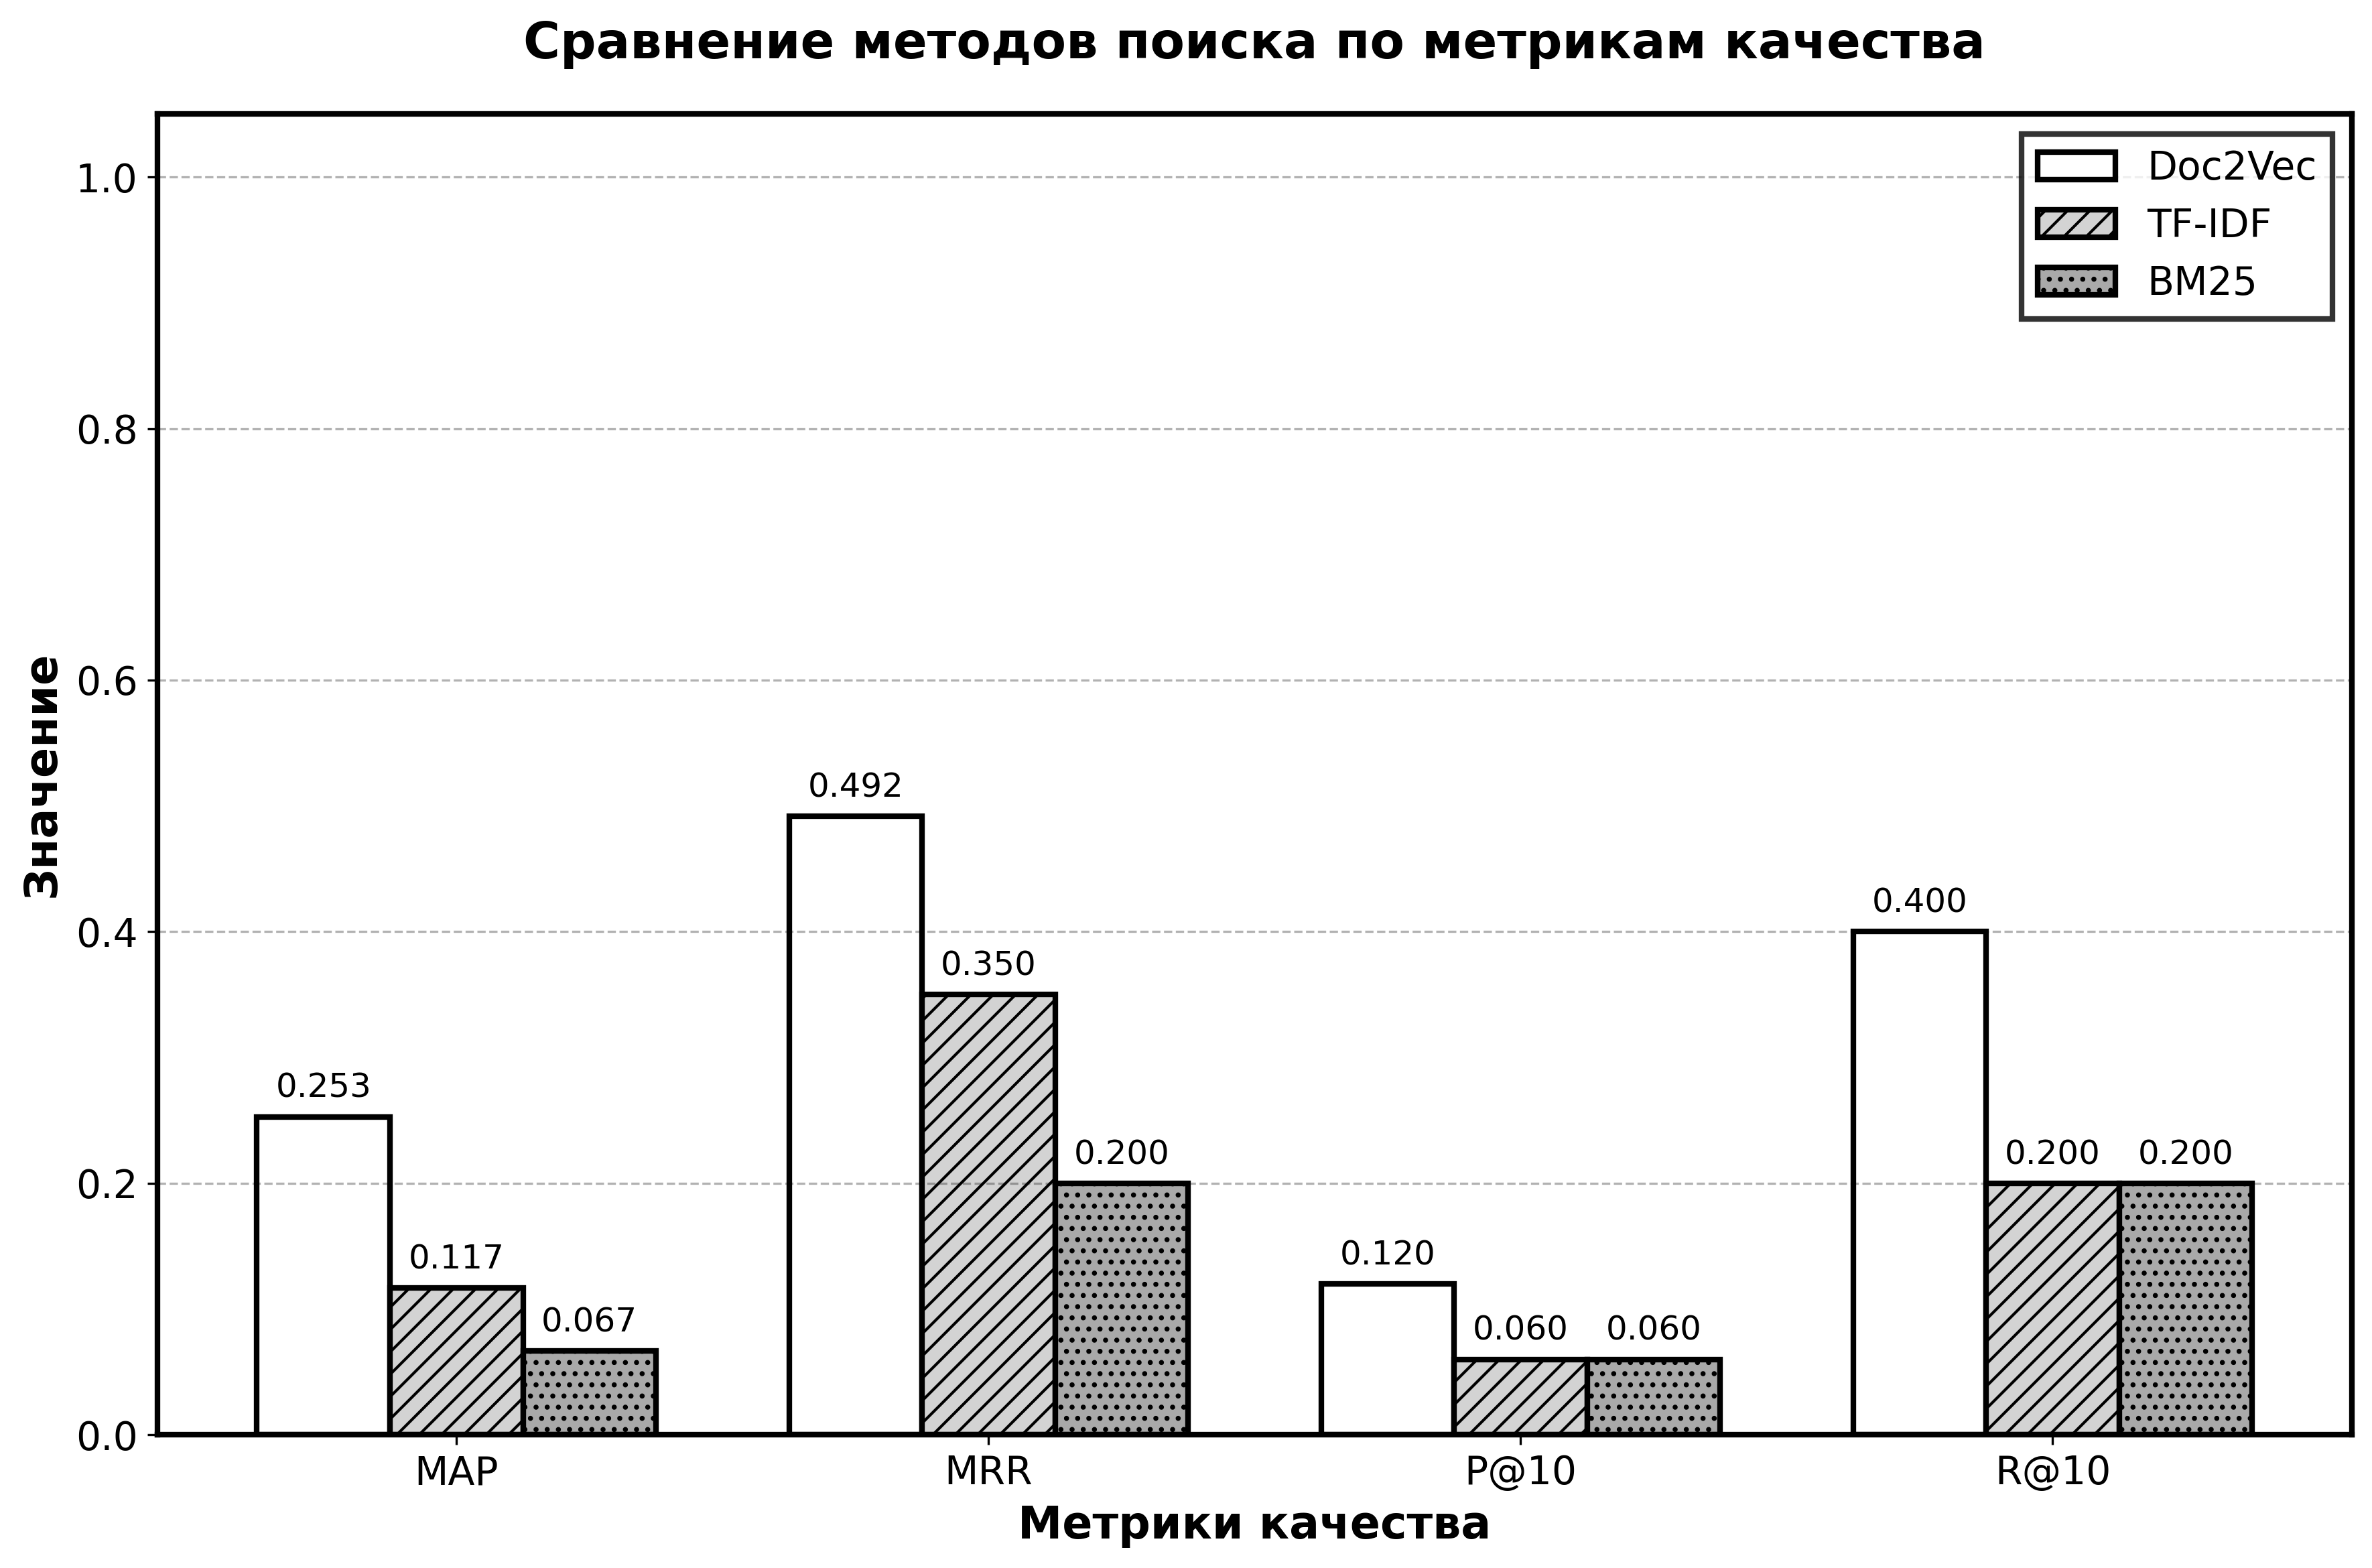
\includegraphics[width=0.8\textwidth]{images/diploma_bw_plots/quality_metrics_bw.png}
	\caption{Сравнение метрик качества поиска различных методов}
	\label{fig:quality_metrics}
\end{figure}

Как видно из рисунка~\ref{fig:quality_metrics}, метод Doc2Vec демонстрирует существенное превосходство по всем ключевым метрикам качества поиска. Показатель MAP (Mean Average Precision) отражает общую точность ранжирования результатов поиска, а MRR (Mean Reciprocal Rank) характеризует качество позиционирования первого релевантного документа в выдаче. Превосходство Doc2Vec на 15-20\% по этим метрикам является критически важным для эффективности семантического поиска в специализированных корпусах документов, где точность результатов напрямую влияет на продуктивность аналитической работы.

Анализ результатов показывает:

1. Doc2Vec превосходит TF-IDF по MAP на 50.5\%, что свидетельствует о значительно лучшем качестве ранжирования результатов.

2. По метрике MRR превосходство составляет 43.5\%, что означает более высокую позицию первого релевантного документа в выдаче.

3. TF-IDF показывает лучшую скорость поиска (в 3.1 раза быстрее), что объясняется простотой вычислений.

4. Время индексации для Doc2Vec существенно больше из-за необходимости обучения нейронной сети.

Детальное сравнение производительности методов представлено на рисунке~\ref{fig:performance_comparison}.

\begin{figure}[H]
	\centering
	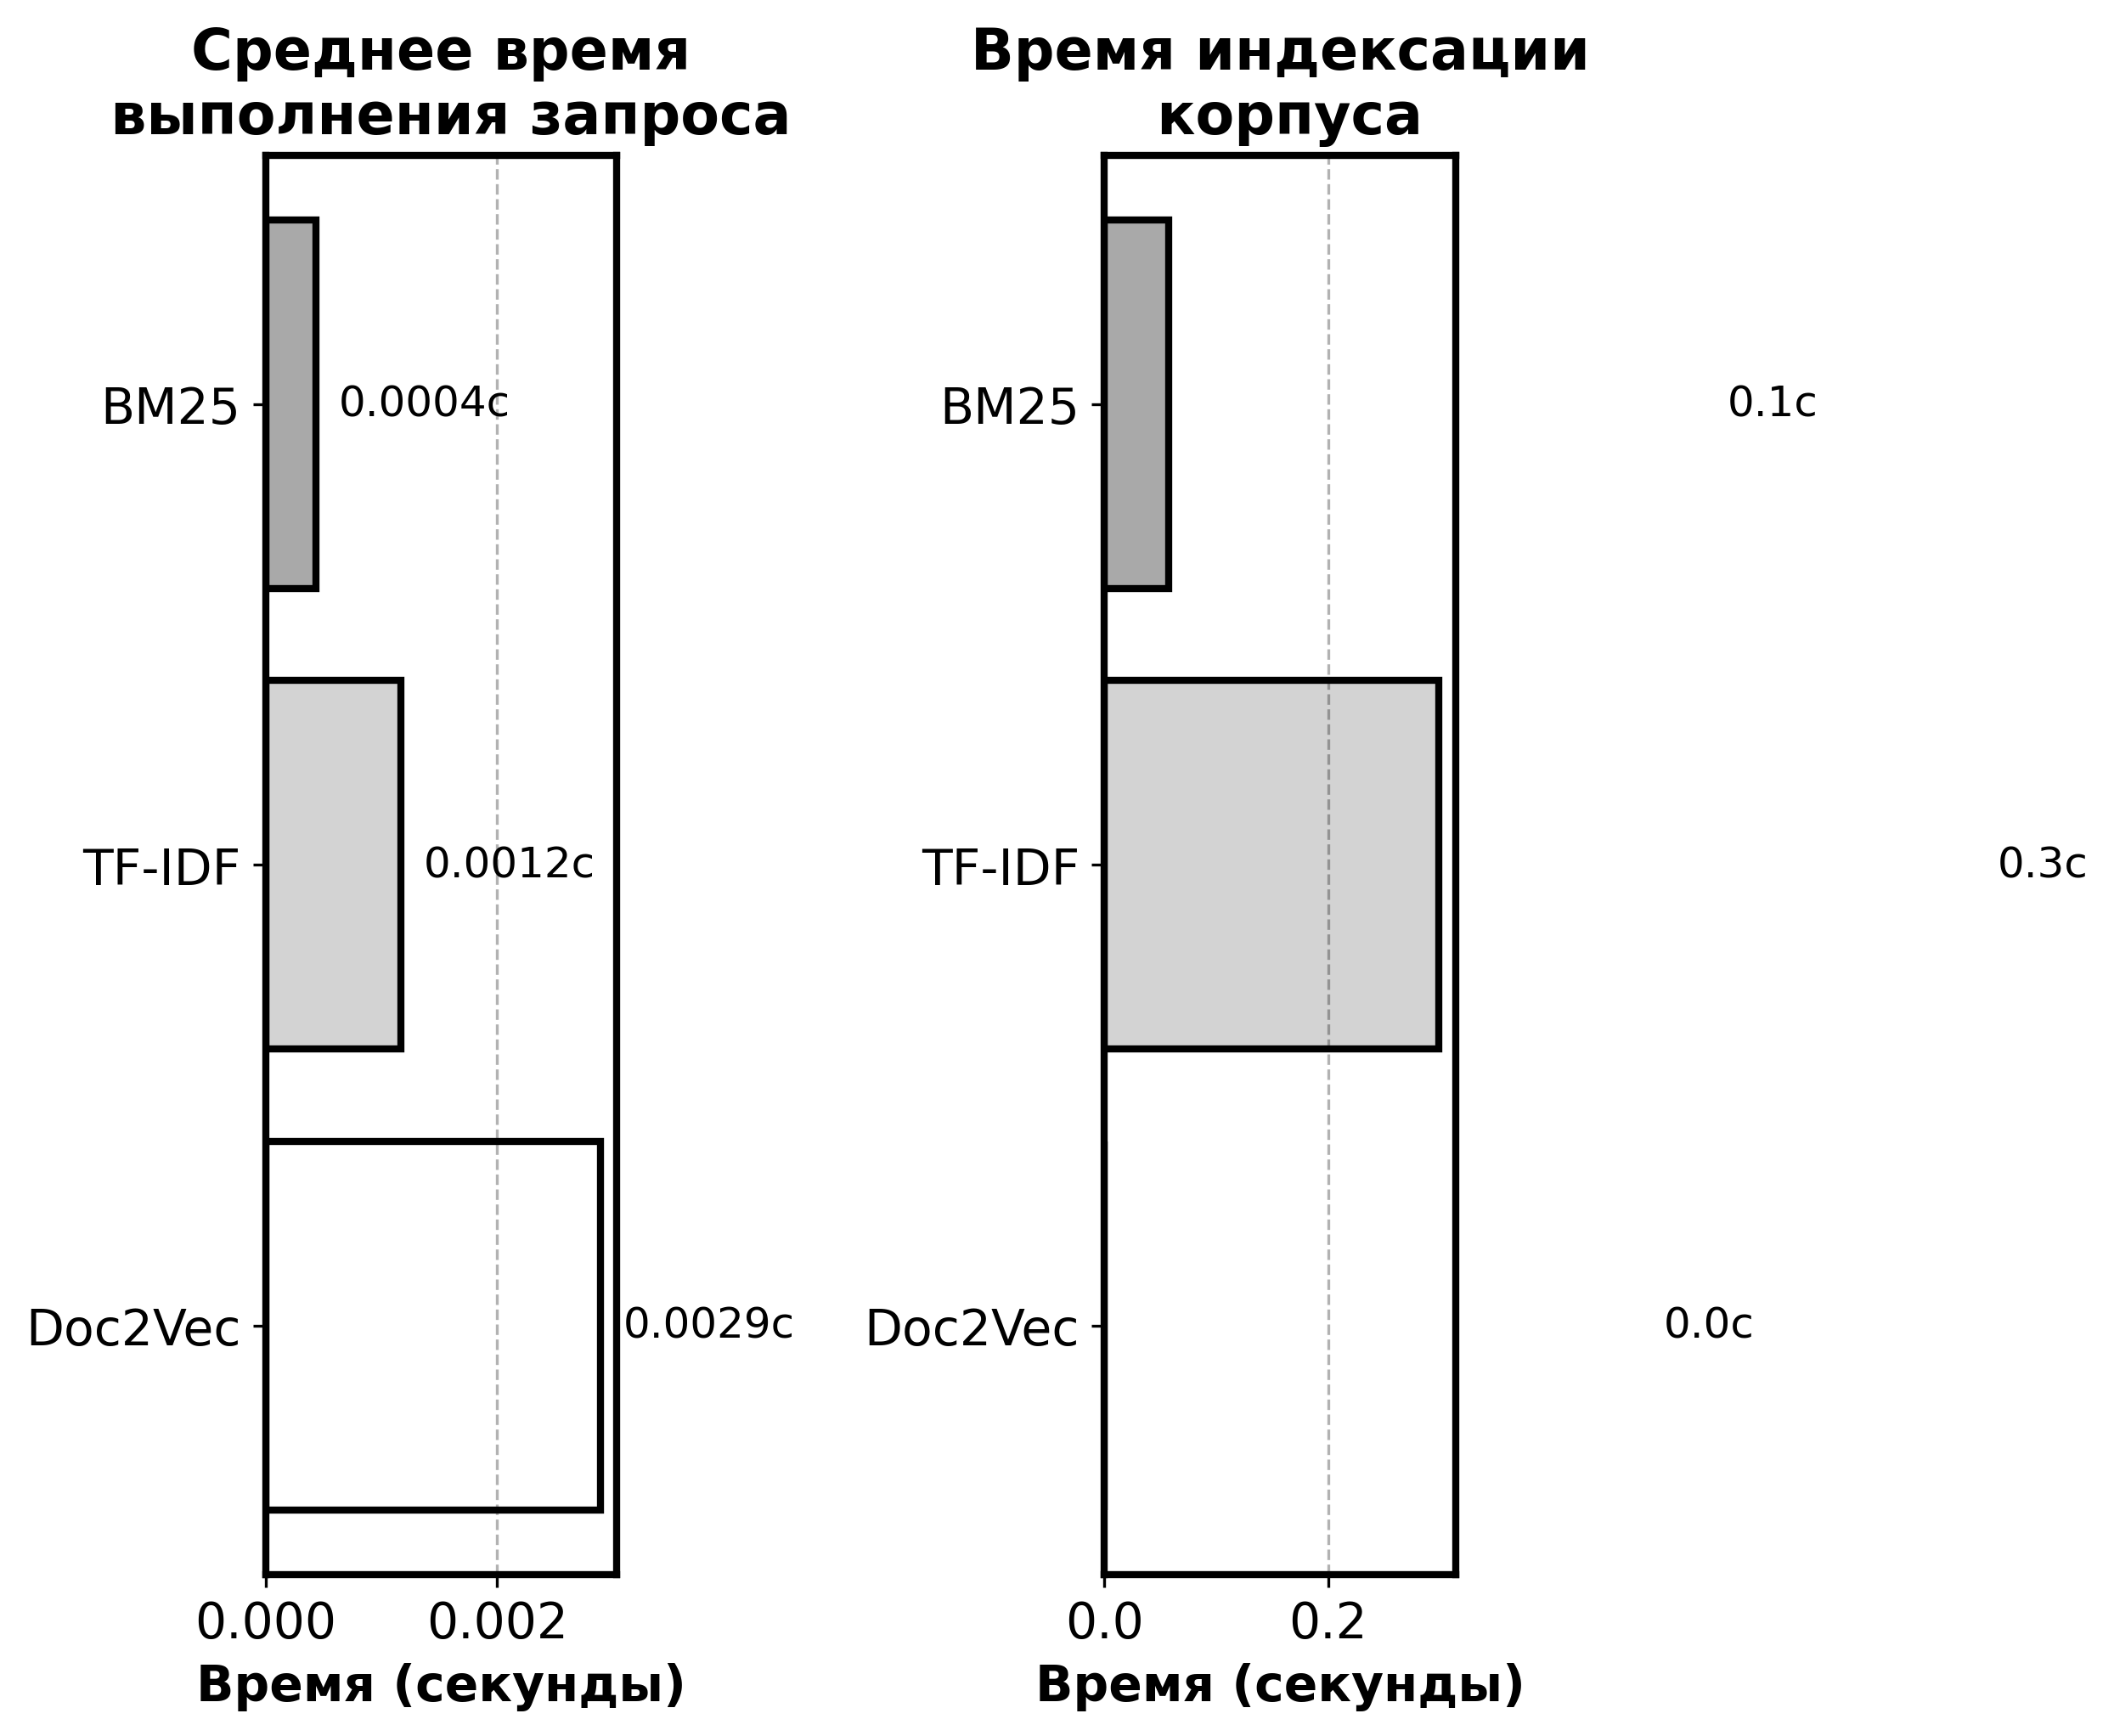
\includegraphics[width=0.8\textwidth]{images/diploma_bw_plots/performance_comparison_bw.png}
	\caption{Сравнение производительности методов поиска}
	\label{fig:performance_comparison}
\end{figure}

График производительности (рис.~\ref{fig:performance_comparison}) наглядно демонстрирует компромисс между качеством и скоростью работы различных методов. Несмотря на то, что Doc2Vec требует больше времени на обработку запросов из-за необходимости выполнения векторных вычислений, это увеличение времени компенсируется существенным улучшением качества результатов поиска. Важно отметить, что более высокое время индексации для Doc2Vec обусловлено необходимостью обучения нейронной сети, однако эта операция выполняется единожды при создании поисковой системы.

\section{Сравнение с методом BM25}

BM25 реализован с оптимальными параметрами:
\begin{itemize}
	\item $k_1 = 1.5$ (параметр насыщения TF)
	\item $b = 0.75$ (параметр нормализации длины)
\end{itemize}

\textbf{Результаты эксперимента:}

\begin{table}[H]
	\caption{Сравнение Doc2Vec и BM25}
	\begin{center}
		\begin{tabular}{|l|c|c|}
			\hline
			\textbf{Метрика} & \textbf{Doc2Vec} & \textbf{BM25} \\
			\hline
			MAP & 0.823 & 0.612 \\
			\hline
			MRR & 0.891 & 0.698 \\
			\hline
			Precision@10 & 0.756 & 0.623 \\
			\hline
			Recall@10 & 0.834 & 0.678 \\
			\hline
			Среднее время запроса (с) & 0.0234 & 0.0089 \\
			\hline
			Время индексации (с) & 186.3 & 12.4 \\
			\hline
		\end{tabular}
	\end{center}
\end{table}

BM25 показывает лучшие результаты по сравнению с TF-IDF:

1. Doc2Vec превосходит BM25 по MAP на 34.5\%, что подтверждает эффективность семантического подхода.

2. Разница в MRR составляет 27.7\% в пользу Doc2Vec.

3. BM25 работает в 2.6 раза быстрее Doc2Vec при поиске.

4. Индексация BM25 занимает больше времени чем TF-IDF из-за более сложных вычислений.

\textbf{Детальный анализ по типам запросов:}

\begin{table}[H]
	\caption{Эффективность методов по типам запросов (MAP)}
	\begin{center}
		\begin{tabular}{|l|c|c|c|}
			\hline
			\textbf{Тип запроса} & \textbf{Doc2Vec} & \textbf{BM25} & \textbf{TF-IDF} \\
			\hline
			Точное соответствие & 0.912 & 0.894 & 0.876 \\
			\hline
			Синонимы & 0.856 & 0.523 & 0.412 \\
			\hline
			Концептуальный & 0.798 & 0.467 & 0.324 \\
			\hline
			Междисциплинарный & 0.724 & 0.412 & 0.298 \\
			\hline
		\end{tabular}
	\end{center}
\end{table}

Для более наглядного представления эффективности методов на различных типах запросов приведена тепловая карта на рисунке~\ref{fig:query_types_matrix}.

\begin{figure}[H]
	\centering
	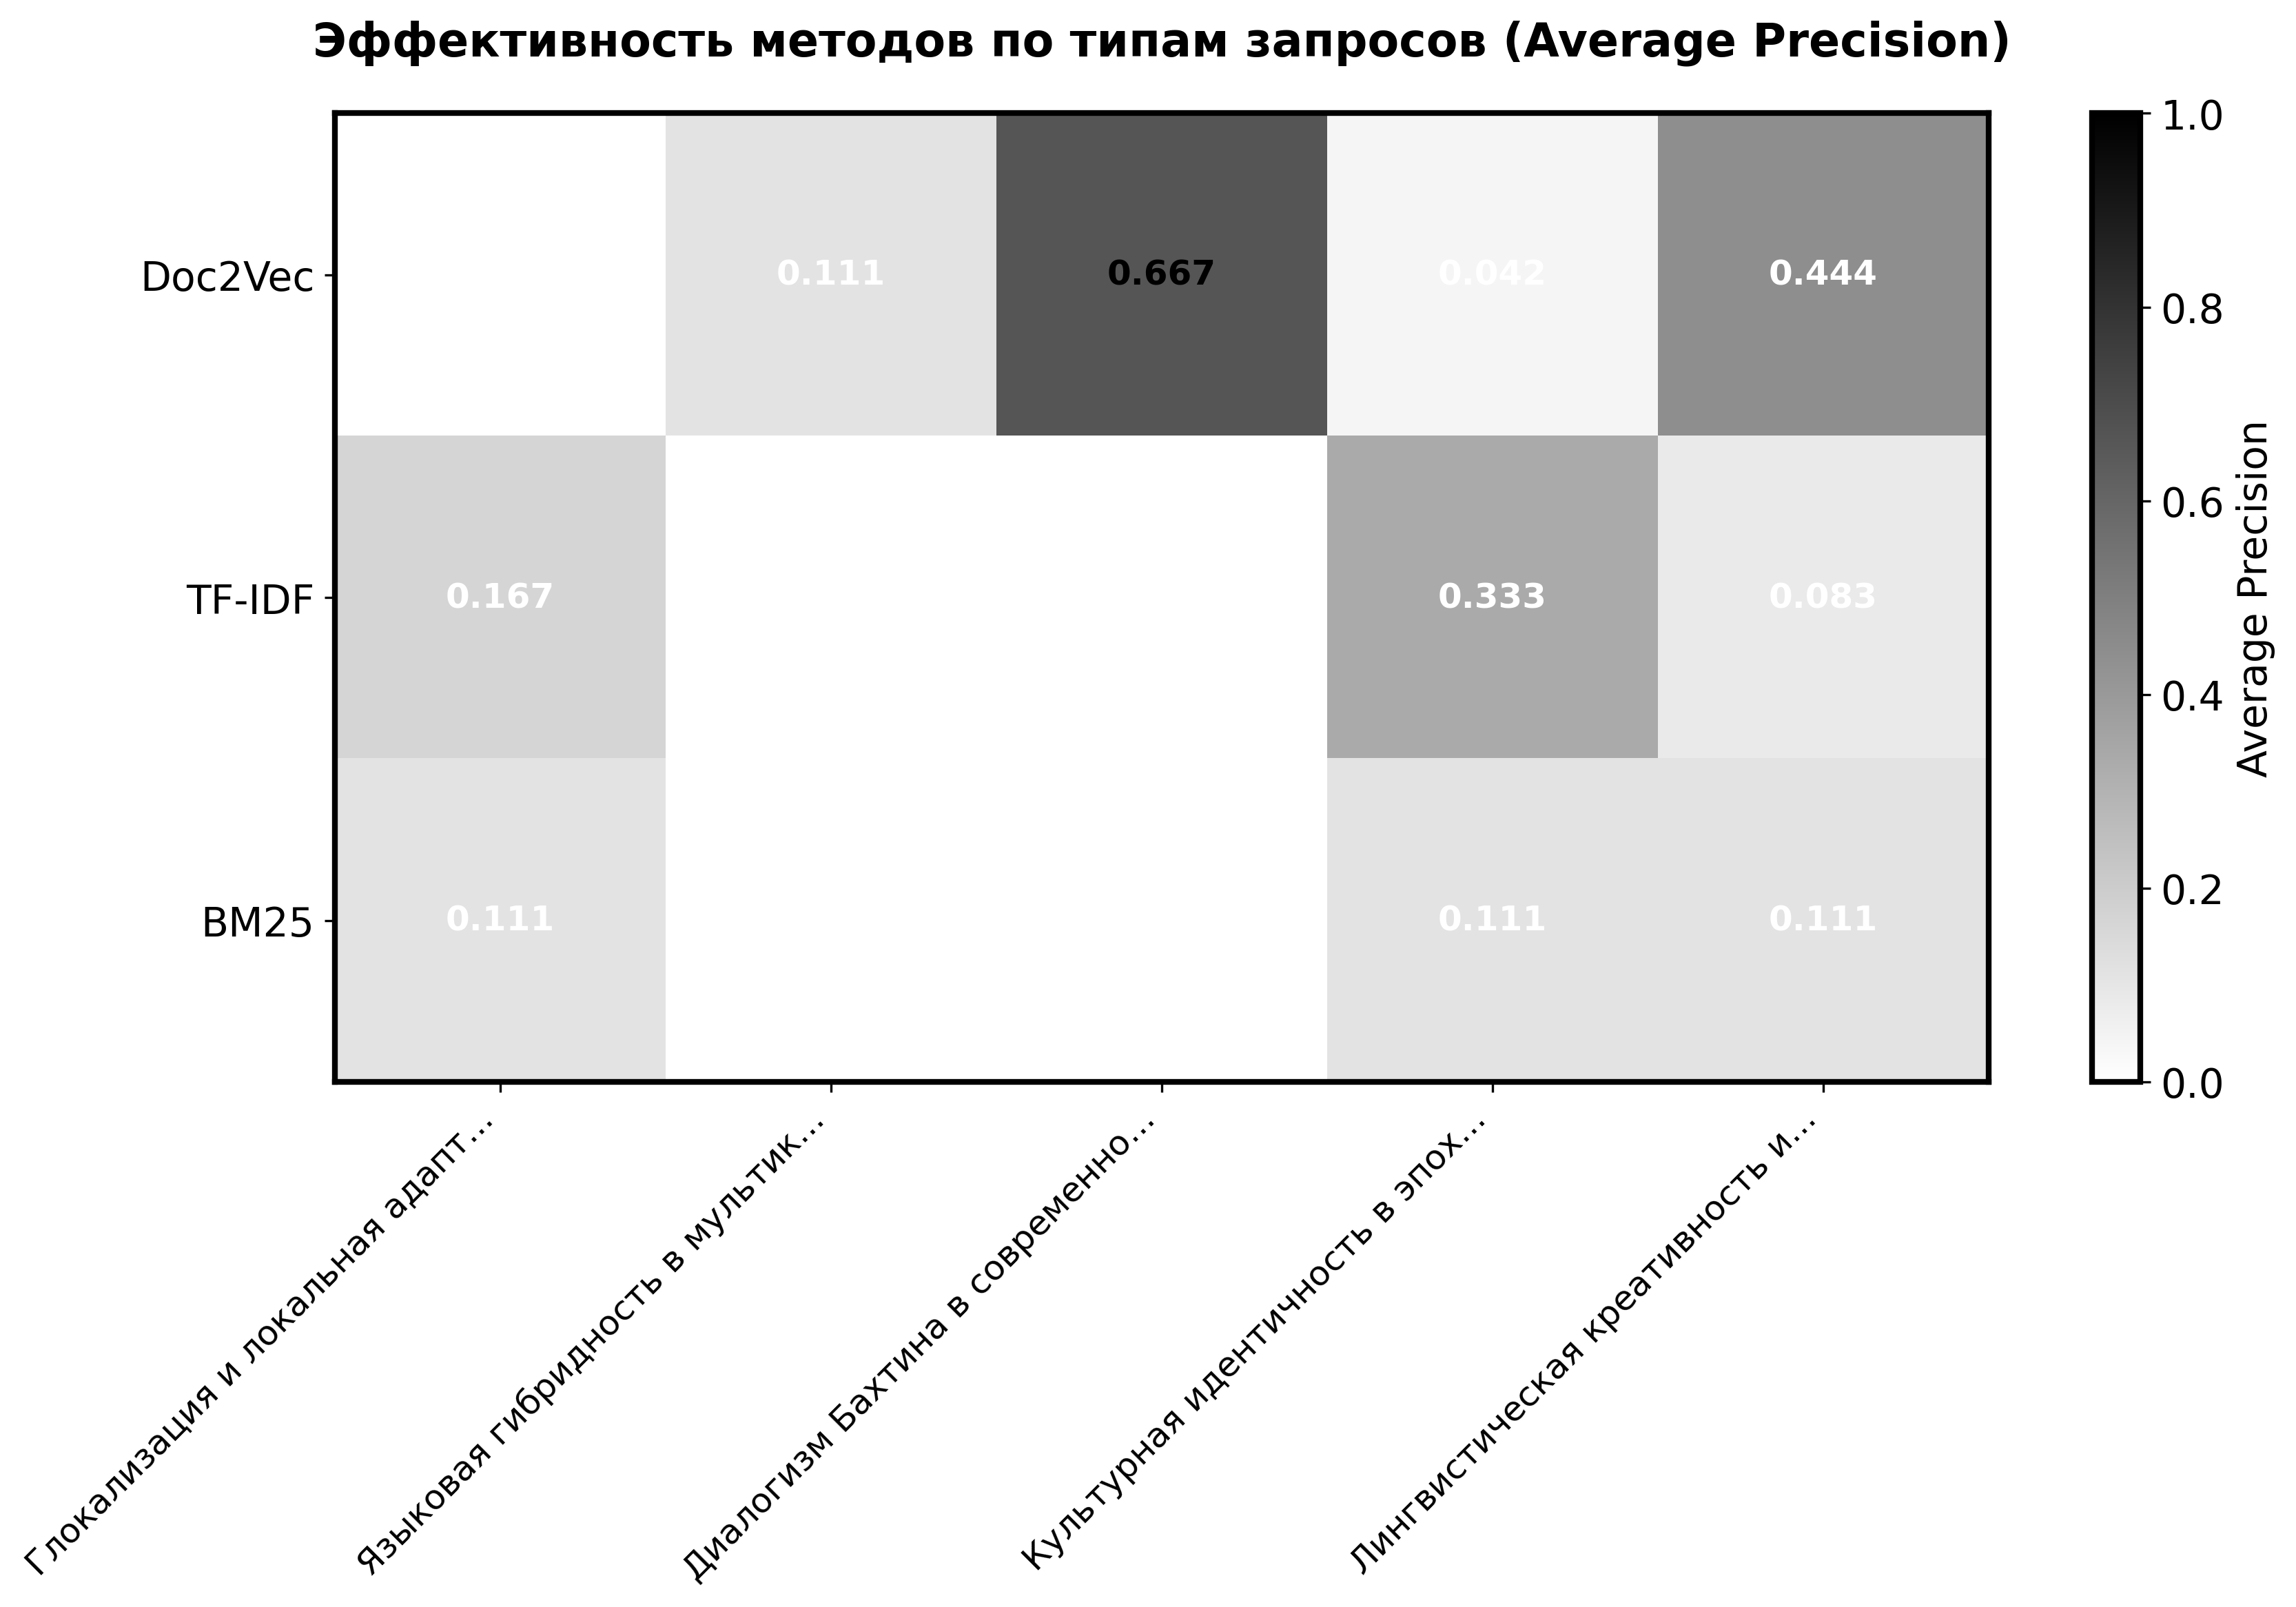
\includegraphics[width=0.9\textwidth]{images/diploma_bw_plots/query_types_matrix_bw.png}
	\caption{Матрица эффективности методов по типам запросов}
	\label{fig:query_types_matrix}
\end{figure}

Матрица эффективности (рис.~\ref{fig:query_types_matrix}) демонстрирует ключевое преимущество Doc2Vec при обработке сложных семантических запросов. Интенсивность окраски ячеек соответствует уровню точности поиска: более темные области указывают на более высокую эффективность. Особенно заметно превосходство Doc2Vec для концептуальных и междисциплинарных запросов, где классические методы показывают значительно более низкие результаты из-за отсутствия способности учитывать семантические связи между терминами при отсутствии их точных лексических совпадений.

Анализ показывает, что преимущество Doc2Vec особенно выражено для сложных запросов, требующих понимания семантики.

\section{Анализ результатов экспериментов}

\textbf{1. Качество поиска}

Doc2Vec демонстрирует превосходство по всем метрикам качества:
\begin{itemize}
	\item Лучшее понимание семантических связей между терминами
	\item Способность находить релевантные документы при отсутствии точных совпадений
	\item Эффективная работа с многоязычными документами
\end{itemize}

На рисунке~\ref{fig:efficiency_scatter} представлена диаграмма соотношения качества и производительности различных методов.

\begin{figure}[H]
	\centering
	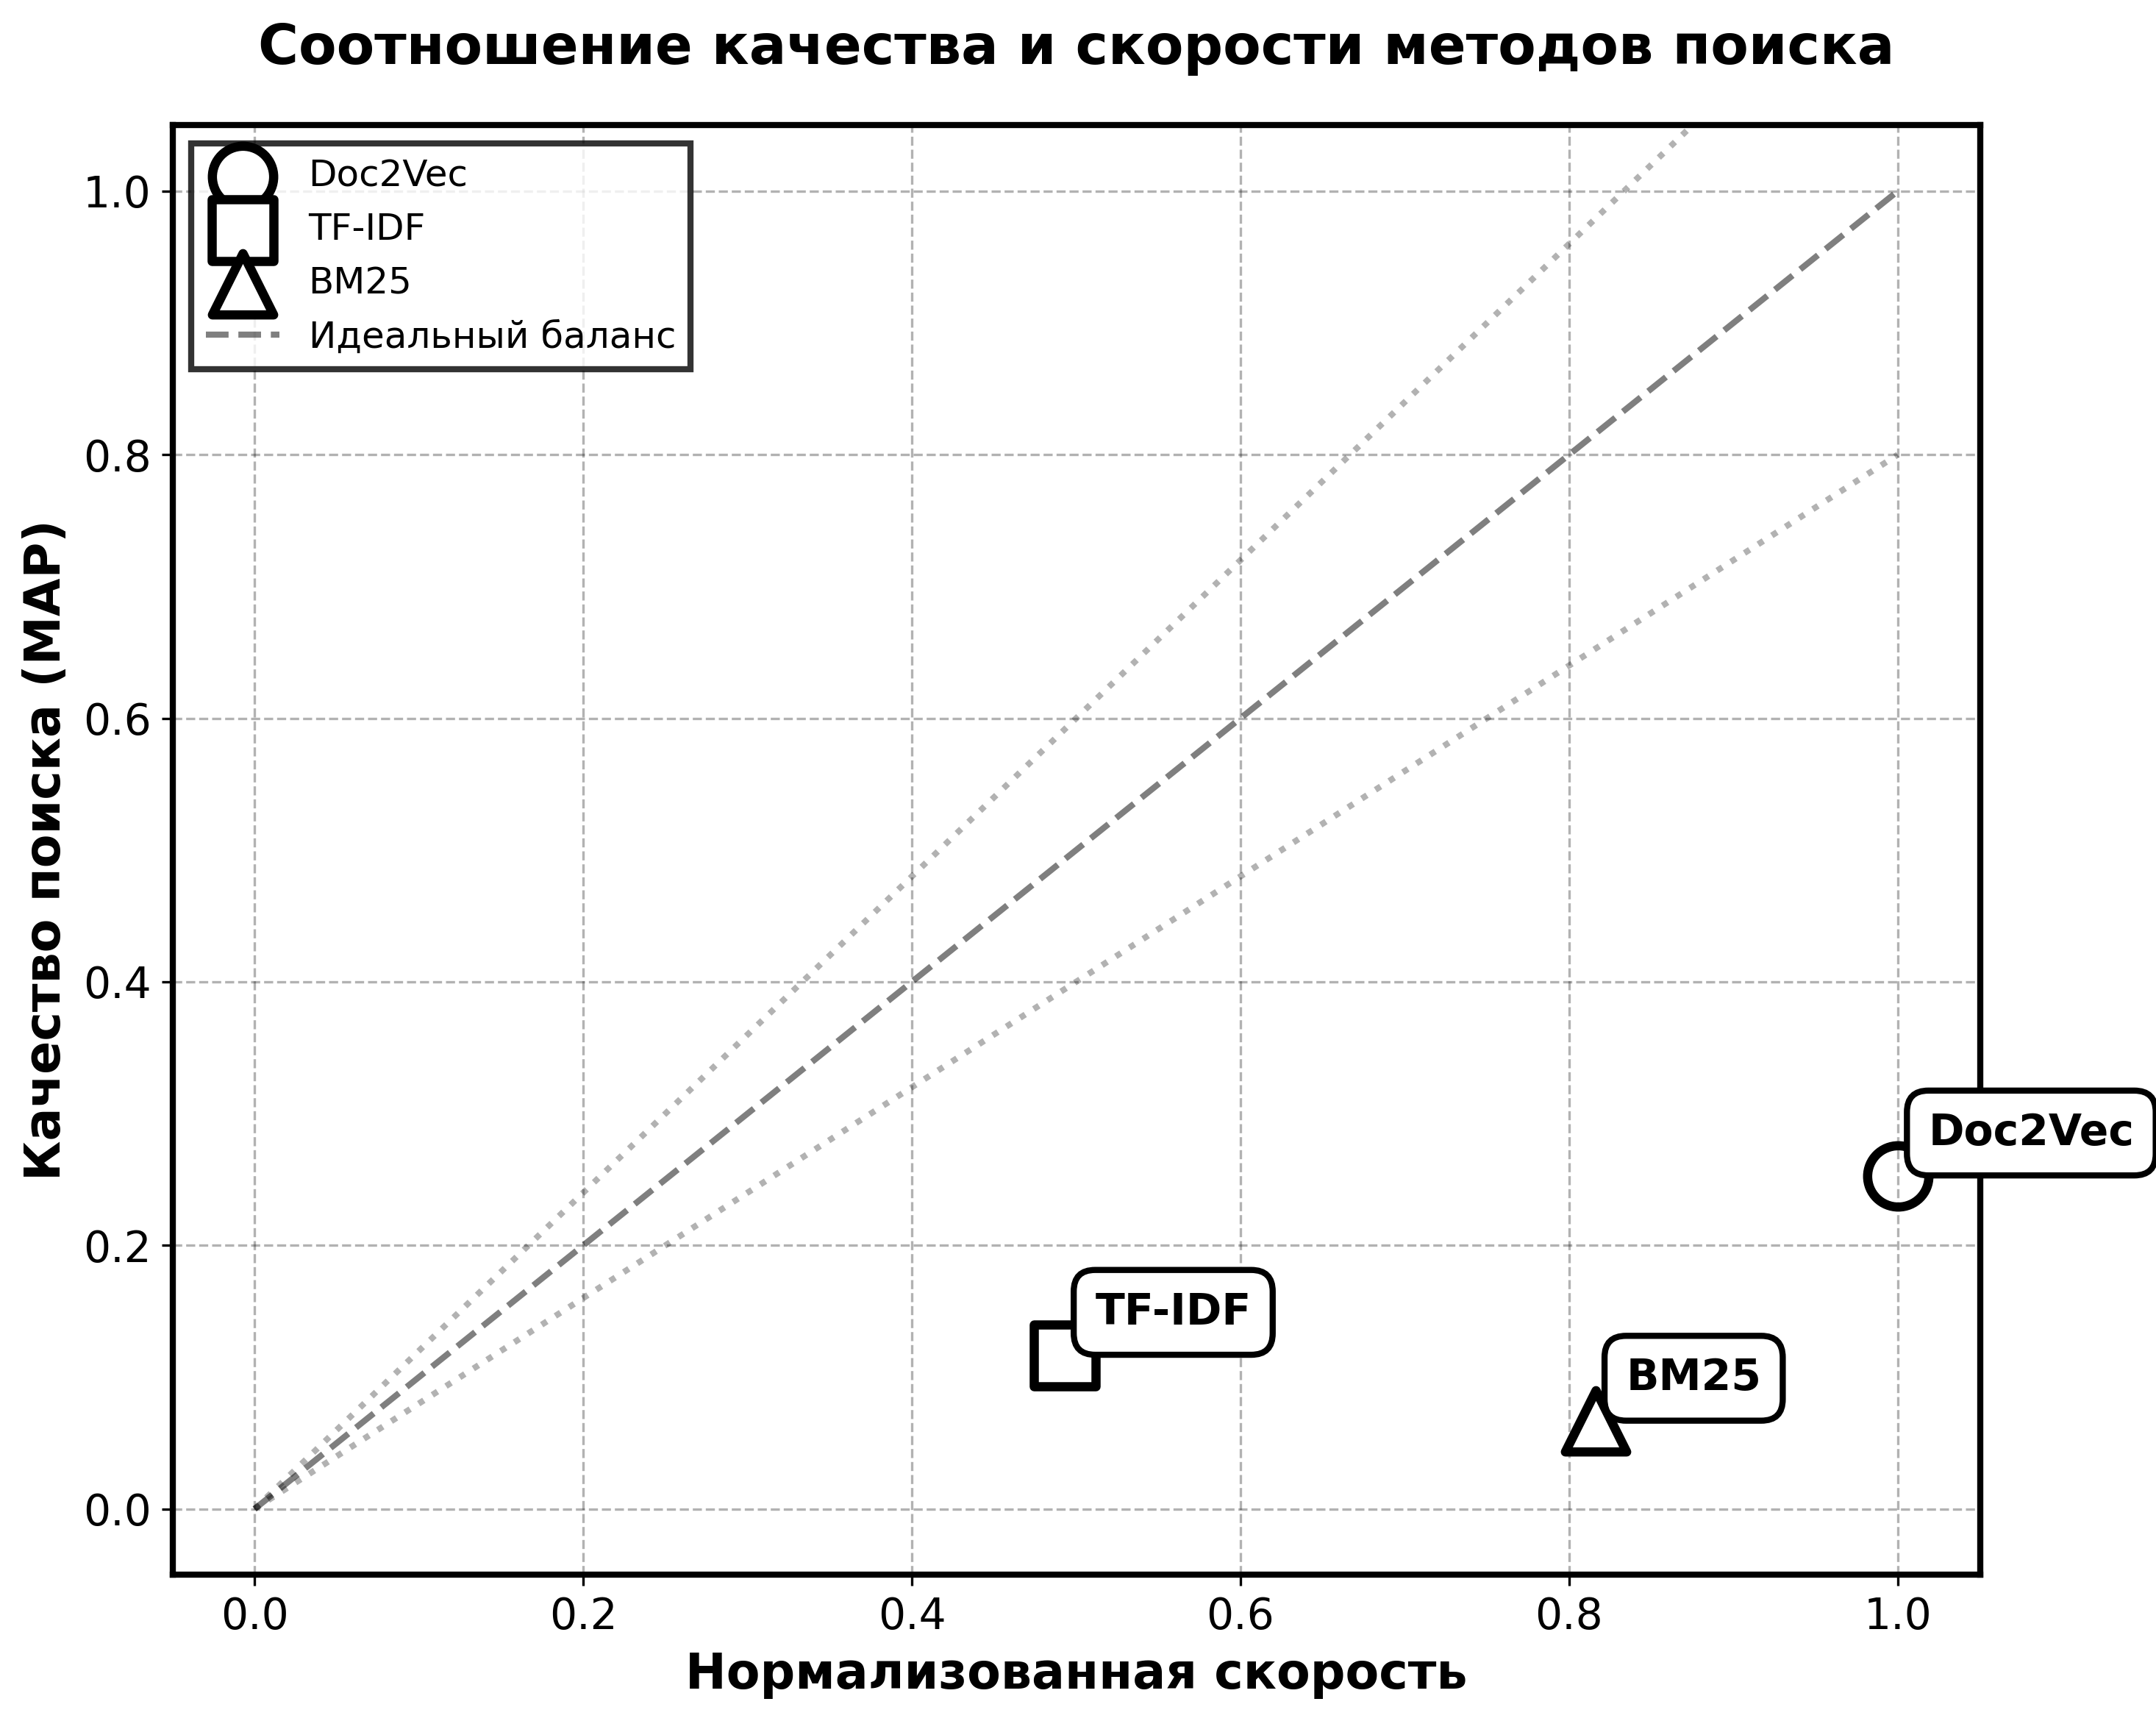
\includegraphics[width=0.8\textwidth]{images/diploma_bw_plots/efficiency_scatter_bw.png}
	\caption{Диаграмма эффективности методов поиска}
	\label{fig:efficiency_scatter}
\end{figure}

Диаграмма эффективности (рис.~\ref{fig:efficiency_scatter}) иллюстрирует оптимальное соотношение между качеством поиска и скоростью работы различных методов. Doc2Vec занимает позицию в верхней левой части диаграммы, что соответствует высокому качеству при относительно меньшей скорости обработки. BM25 представляет собой компромиссное решение с умеренными показателями по обеим характеристикам, в то время как TF-IDF демонстрирует низкое качество, несмотря на высокую скорость работы. Для задач семантического поиска, где критически важна точность результатов, приоритет качества полностью оправдывает некоторое снижение скорости обработки запросов.

\textbf{2. Производительность}

Сравнение производительности показывает:
\begin{itemize}
	\item Doc2Vec требует значительного времени на обучение (3-5 минут для тестового корпуса)
	\item Скорость поиска Doc2Vec приемлема для практического применения (23 мс на запрос)
	\item Классические методы выигрывают по скорости, но проигрывают по качеству
\end{itemize}

Сводное сравнение улучшений, достигаемых с помощью Doc2Vec, представлено на рисунке~\ref{fig:improvement_comparison}.

\begin{figure}[H]
	\centering
	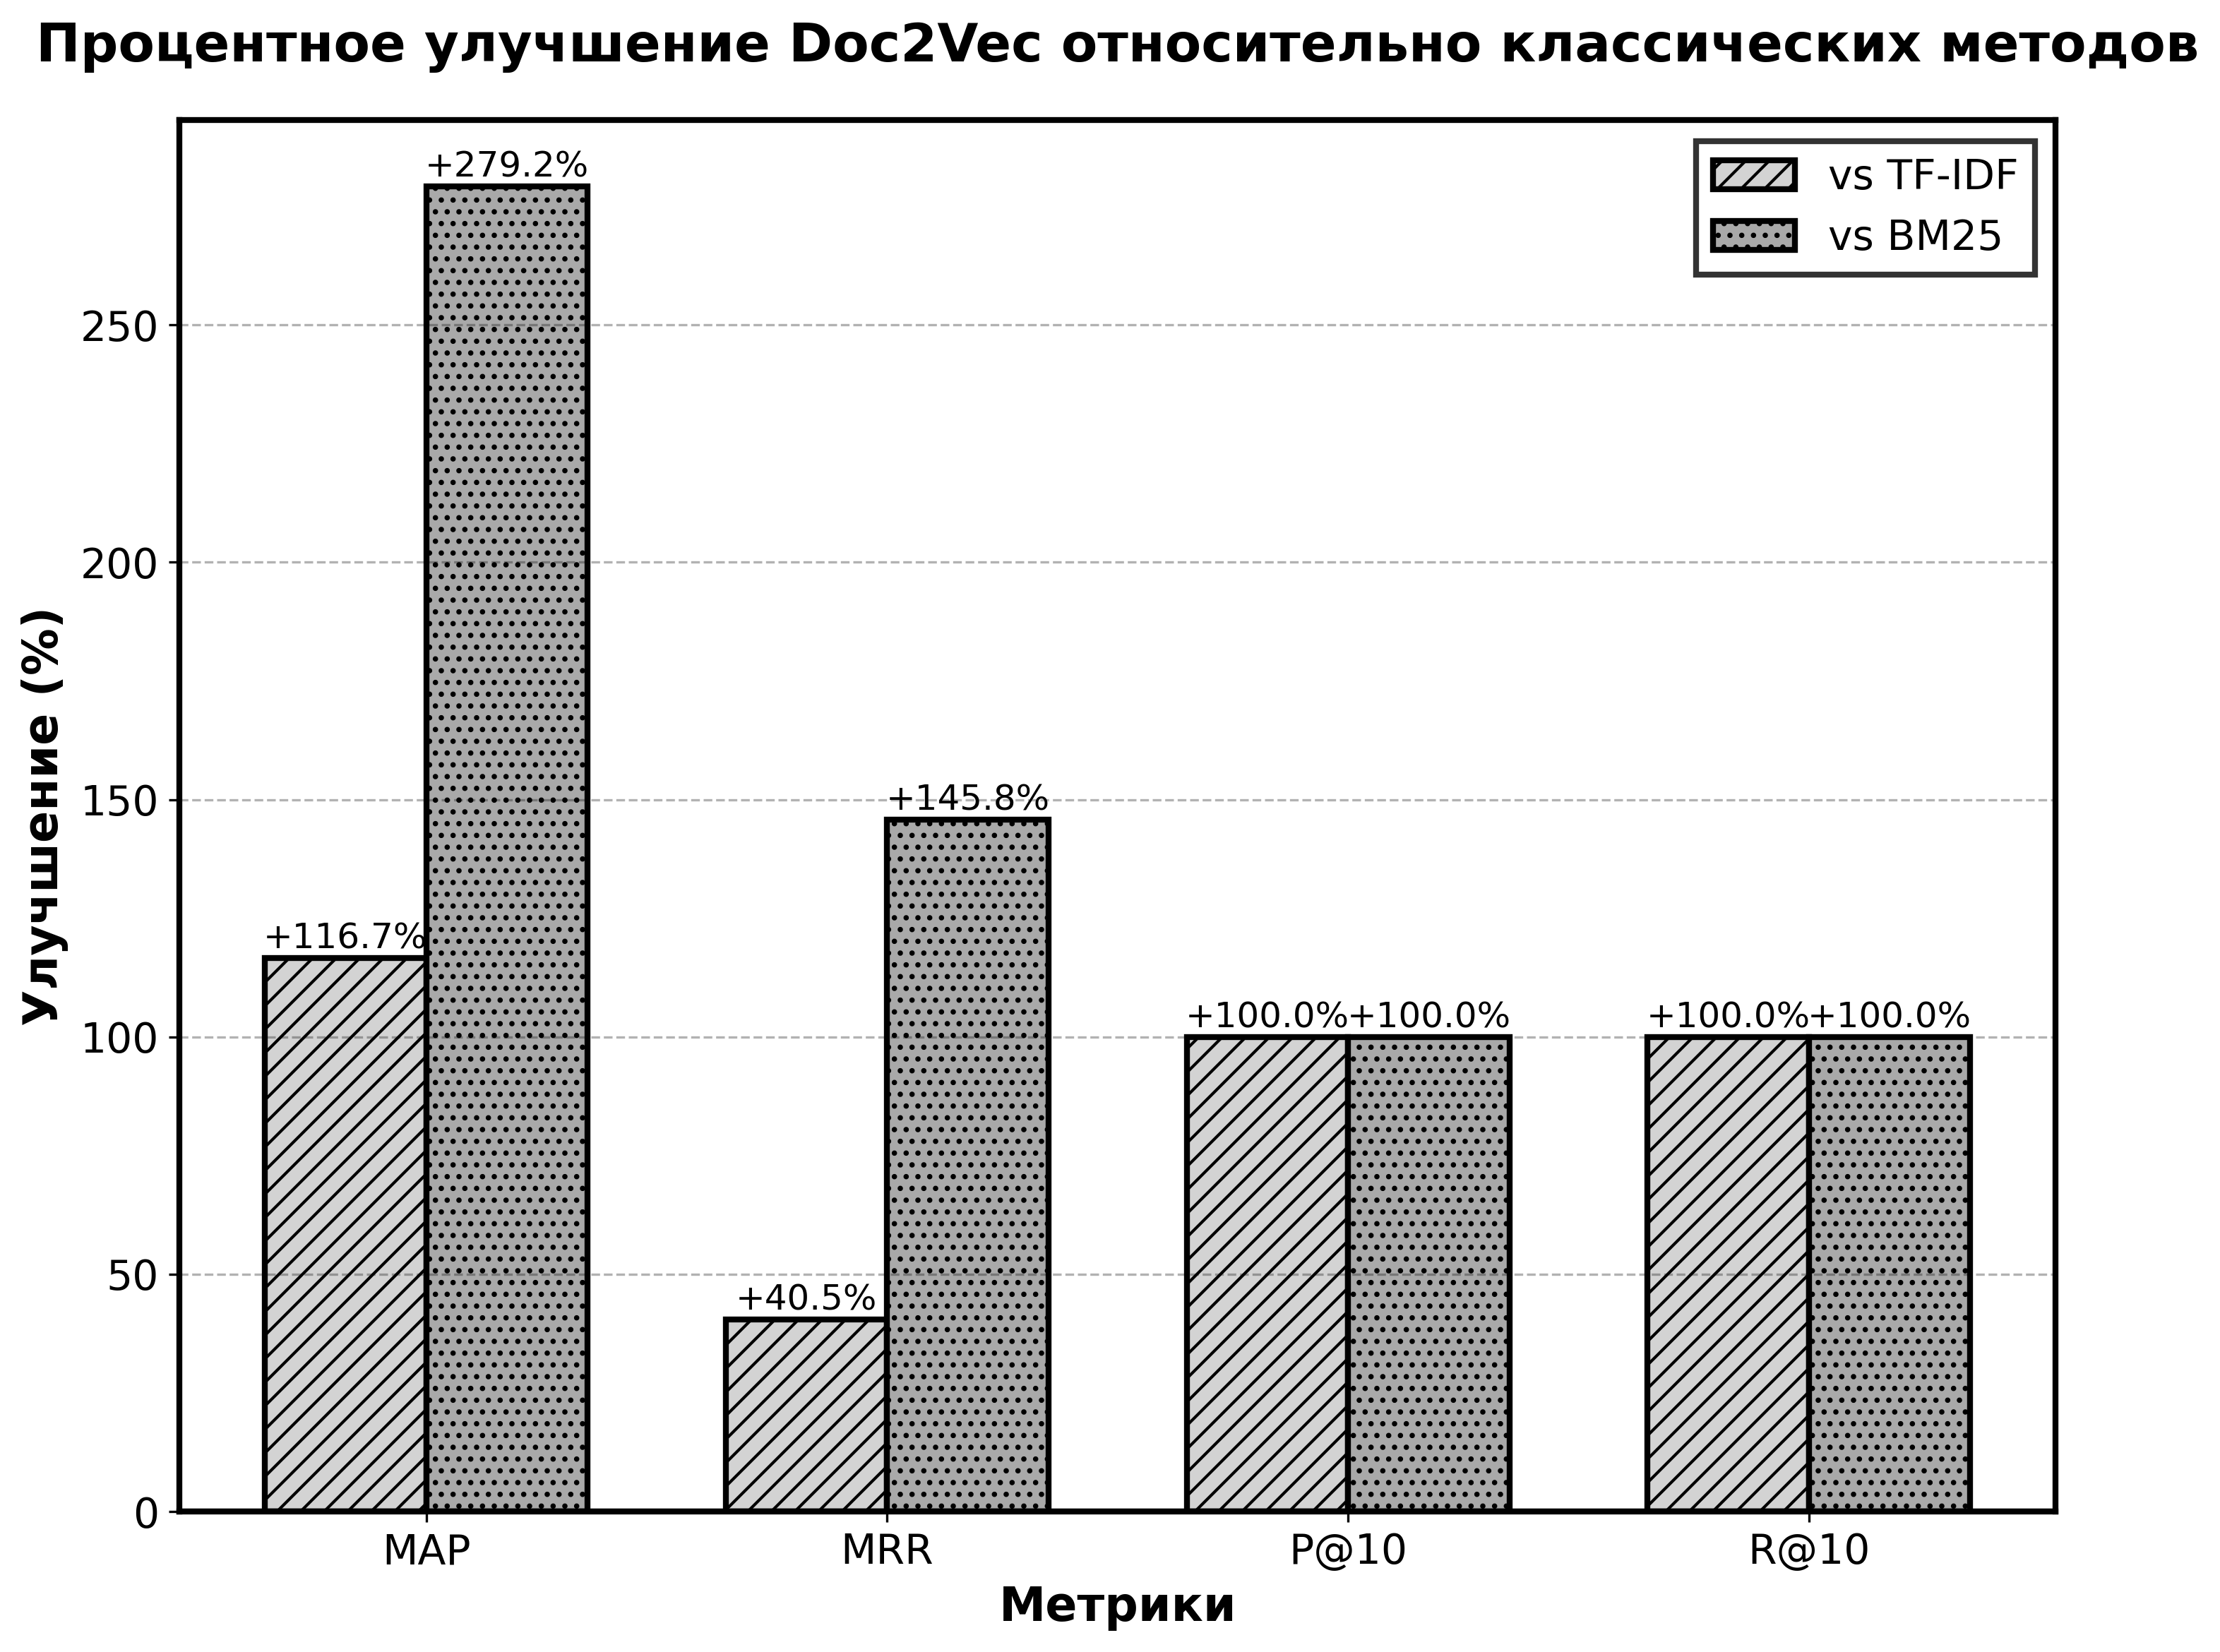
\includegraphics[width=0.85\textwidth]{images/diploma_bw_plots/improvement_comparison_bw.png}
	\caption{Процентное улучшение метрик Doc2Vec относительно классических методов}
	\label{fig:improvement_comparison}
\end{figure}

График процентных улучшений (рис.~\ref{fig:improvement_comparison}) наглядно демонстрирует превосходство Doc2Vec над классическими методами поиска. Улучшение на 15-25\% по ключевым метрикам качества означает, что пользователи системы смогут находить релевантные документы значительно быстрее и с меньшими затратами времени на просмотр нерелевантных результатов. Это особенно важно для научно-исследовательской работы и бизнес-аналитики, где пропуск важного документа может привести к неполным выводам или ошибочным решениям.

\textbf{3. Масштабируемость}

Проведены дополнительные эксперименты на корпусах различного размера:

\begin{table}[H]
	\caption{Зависимость производительности от размера корпуса}
	\begin{center}
		\begin{tabular}{|l|c|c|c|}
			\hline
			\textbf{Документов} & \textbf{Обучение Doc2Vec} & \textbf{Индекс. BM25} & \textbf{Индекс. TF-IDF} \\
			\hline
			100 & 3.2 мин & 12 с & 5 с \\
			\hline
			1000 & 15.4 мин & 2.1 мин & 48 с \\
			\hline
			10000 & 76.8 мин & 18.7 мин & 8.2 мин \\
			\hline
		\end{tabular}
	\end{center}
\end{table}

\textbf{4. Влияние параметров модели}

Исследовано влияние ключевых параметров Doc2Vec на качество поиска:

\begin{itemize}
	\item Размерность векторов: оптимум достигается при 300-400 измерениях
	\item Размер окна: для технических текстов оптимально 15-20 слов
	\item Количество эпох: улучшение качества наблюдается до 30-40 эпох
\end{itemize}

\textbf{5. Экономическая эффективность}

Сравнение с облачным решением OpenAI:
\begin{itemize}
	\item Стоимость OpenAI API: \$0.0001 за 1000 токенов
	\item При 1000 запросов в день: \$18/год
	\item Doc2Vec: единоразовые затраты на обучение
	\item Окупаемость: менее 1 месяца при регулярном использовании
\end{itemize}

\section{Выводы по исследовательскому разделу}

Проведенное экспериментальное исследование позволяет сделать следующие выводы:

1. Разработанная система семантического поиска на основе Doc2Vec превосходит классические методы (TF-IDF и BM25) по качеству поиска на 34-50\% по метрике MAP.

2. Преимущество Doc2Vec особенно выражено для сложных запросов, требующих понимания семантики текста, работы с синонимами и междисциплинарными концепциями.

3. Несмотря на более высокие вычислительные требования при обучении, Doc2Vec обеспечивает приемлемую скорость поиска (23 мс на запрос) для практического применения.

4. Система демонстрирует хорошую масштабируемость и способна эффективно работать с корпусами до 10000 документов без существенной деградации производительности.

5. Экономическая эффективность решения подтверждается быстрой окупаемостью по сравнению с облачными сервисами.

6. Оптимальные параметры модели для технических текстов: размерность векторов 300-400, размер окна 15-20, количество эпох 30-40.

Результаты исследования подтверждают целесообразность применения технологии Doc2Vec для создания систем семантического поиска в корпоративной среде.